% load the document class
\documentclass[]{biophysicist}

% define title information
\title[PHYS 495 Report Draft]{PHYS 495 Report Draft: Title in Progress}

% define author information
\author{Calvin Sprouse}{cwu}
\affiliation{cwu}{Central Washington Universtiy Department of Physics, Ellensburg, Washington, 98926}
\date[2019]{Received = 1st July 2020, Published = 8th September 2020}

% import packages
\usepackage{kantlipsum}
\usepackage{booktabs}

% begin document
\begin{document}

% create the abstract block
\begin{abstract}
Disruption of axonal microtubule (MT) arrays is a key factor in nerve degeneration associated with neurodegenerative diseases such as Alzheimer's. In developing axons, nearly all MTs are oriented with their plus ends away from the cell body, referred to as a “plus-end-out” polarity pattern. This uniform polarity pattern is under continual threat of corruption in the face of nucleation of new MTs and “flipping” of short MTs into a minus-end-out orientation. Here, we present a computational study using agent-based simulations and visual animations to demonstrate how the self-organizing properties of the cytoskeleton contribute to the establishment and maintenance of the MT polarity pattern in axons. We show that occasional minus-end-out MTs can be cleared from the axon through a “polarity sorting” mechanism in which cytoplasmic dynein slides anti-parallel MTs with their plus-ends leading. We identify conditions under which a simple dynein-based polarity-sorting mechanism is insufficient to prevent MT polarity flaws from accumulating. Our simulations exhibit a positive feedback loop that emerges when mis-oriented MTs grow and incorporate into the MT array, and in turn undermine the efficiency of motor-based polarity-sorting in clearing new minus-end-out MTs from the axon. We hypothesize that a static crosslinking protein, such as TRIM46, which resists relative sliding between parallel MTs plays an essential role in “error prevention” by stabilizing the plus-end-out MT array while allowing dynein-based polarity sorting to remove occasional minus-end-out MTs. We further hypothesize that another static crosslinker, such as PRC1, may boost the efficiency of polarity sorting by aligning anti-parallel MTs to facilitate dynein-based sliding. Initial experiments demonstrate that inhibition of these candidate crosslinking proteins produces an increase in MT polarity flaws in vertebrate axons, in support of our model for a multiple-player polarity-sorting mechanism in the axonal MT array.
\end{abstract}

% create the keywords block
\keywords{computational, simulations, microtubules, neurons, axons}

% paste the title information
\maketitle

% introduction and background, taken from wa-aapt_poster
\section{Introduction}
Disruption of axonal microtubule (MT) arrays is a key factor in nerve degeneration associated with neurodegenerative diseases such as Alzheimer’s. In developing axons, nearly all MTs are oriented with their plus ends away from the cell body, referred to as a “plus-end-out” polarity pattern. This uniform polarity pattern is under continual threat of corruption in the face of nucleation of new MTs and ``flipping'' of short MTs into a minus-end-out orientation. Computational investigation of how self-organizing properties of the cytoskeleton contribution to the establishment and maintenance of the MT polarity pattern in axons. MT movement is dependent on the relative arrangements of motor proteins and MT pairs, as well as the presence of crosslinking proteins.

\begin{figure}
    \centering
    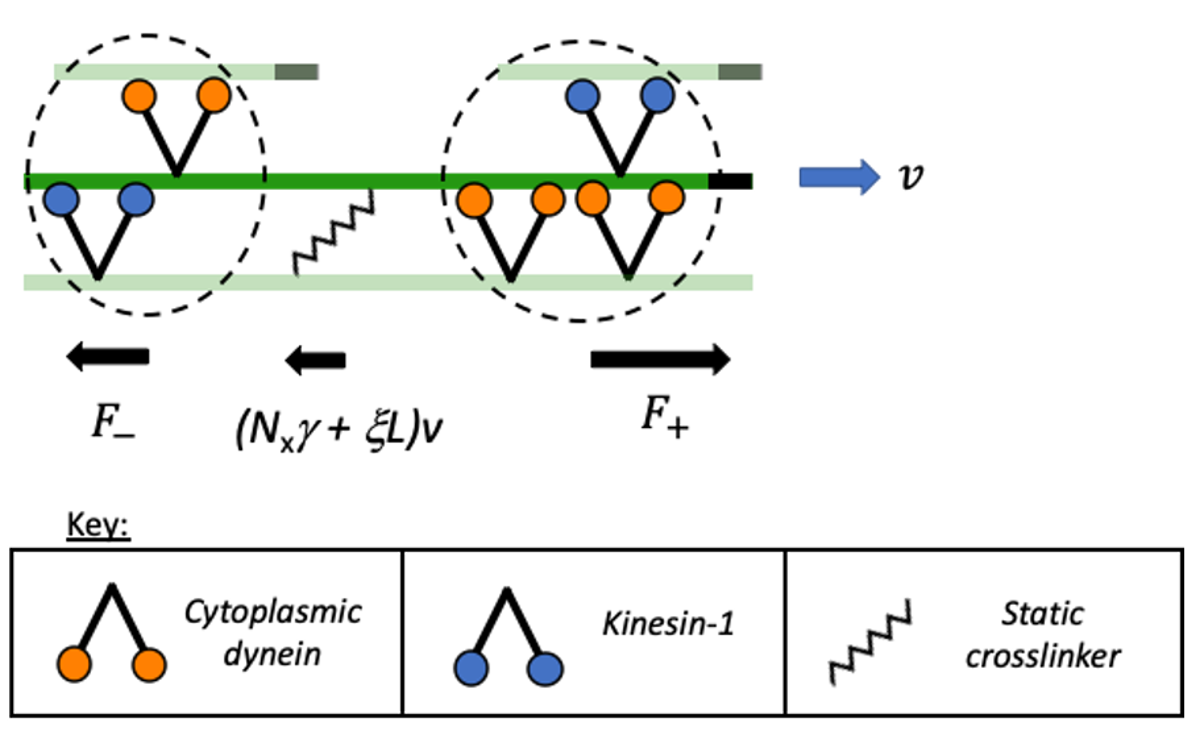
\includegraphics[width=0.4\textwidth]{figures/model1.png}
    \caption{The forces exerted on microtubules are dependent on the relative orientation and type of motors bound.}
    \label{fig:mtmovement}
\end{figure}

Shown in Figure \ref{fig:mtmovement} are representative modes of microtubule movement.
% here I will talk more about our focus on dynein specifically, there was an excellent figure that we used for dynein sliding from a previous model section

% methods and models section
\section{Methods}
To investigate motor based polarity sorting we use agent-based simulations.
\begin{equation}
    \frac{\text{d}N}{\text{d}{t}} = r_{\text{d,on}} - r_{\text{d,off}} N_{\text{d}}
\end{equation}
The simulation is based on a force balance equation. We model the cellular fluid as being so viscous that MTs not being actively pushed by motors are stopped instantly. This results in an environment where MTs move with near constant velocities determined by the number and type of attached motors and otherwise remain at rest.

Describe the method of polarity sweeps.

We use animated visualizations of simulations to better approach an understanding of the behavior in the axon. These animations are produced in Python after the corresponding simulation has finished running.

% results
\section{Results}
Using the simulations has allowed for debugging, while that wouldnt show up in a paper that would absolutely be important in a project report. So far the animations have addressed some ``deleting'' inconsistencies, MTs would be deleted when touching the cell body. They have also addressed some issues in re-spawning MTs without updating their length. All things that could easily go unnoticed since who would think to look for them.

We observe many complex interdependencies between simulation parameters.
\begin{figure}
    \centering
    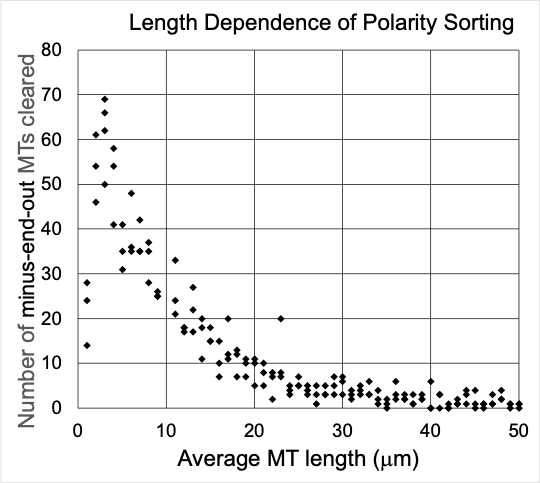
\includegraphics[width=0.4\textwidth]{figures/length_dependence.png}
    \caption{The length dependence on polarity sorting. Clearing more minus-end-out MTs is good.}
    \label{fig:lengthdep}
\end{figure}
By varying the average MT length we observe, up to a point, that for all other parameters being equal shorter MTs allow for better polarity sorting action. This is due to short MTs being more motile within the axon. Longer MTs tend to acquire a higher proportion of molecular motors creating ``tug-of-war'' problems leading to mostly stationary behavior. This is good for polarity sorting behavior if the stationary MTs are plus-end-out but not good if they are minus-end-out.

% discussion
\section{Discussion}
Talk about the impact of these complex parameter relationships.

% sliding and axon growth
\section{Next Steps}
Realistically I need to work this into the abstract for my report since it will eventually be part of my model and results.

It is well established that MT play a \textit{signaling} role in axon growth: conveying chemical cues to the axon structure to engage or disengage a ``clutch'' mechanism. To determine whether MTs also play a role in pushing the growth cone forward during axonal elongation, we will: (1) determine the magnitude of force between the axonal MT array and the growth cone, arising from motor-based sliding of MTs; and (2) compare this force with measured traction forces between growth cones and their substrates during axonal growth.

\begin{figure}
    \centering
    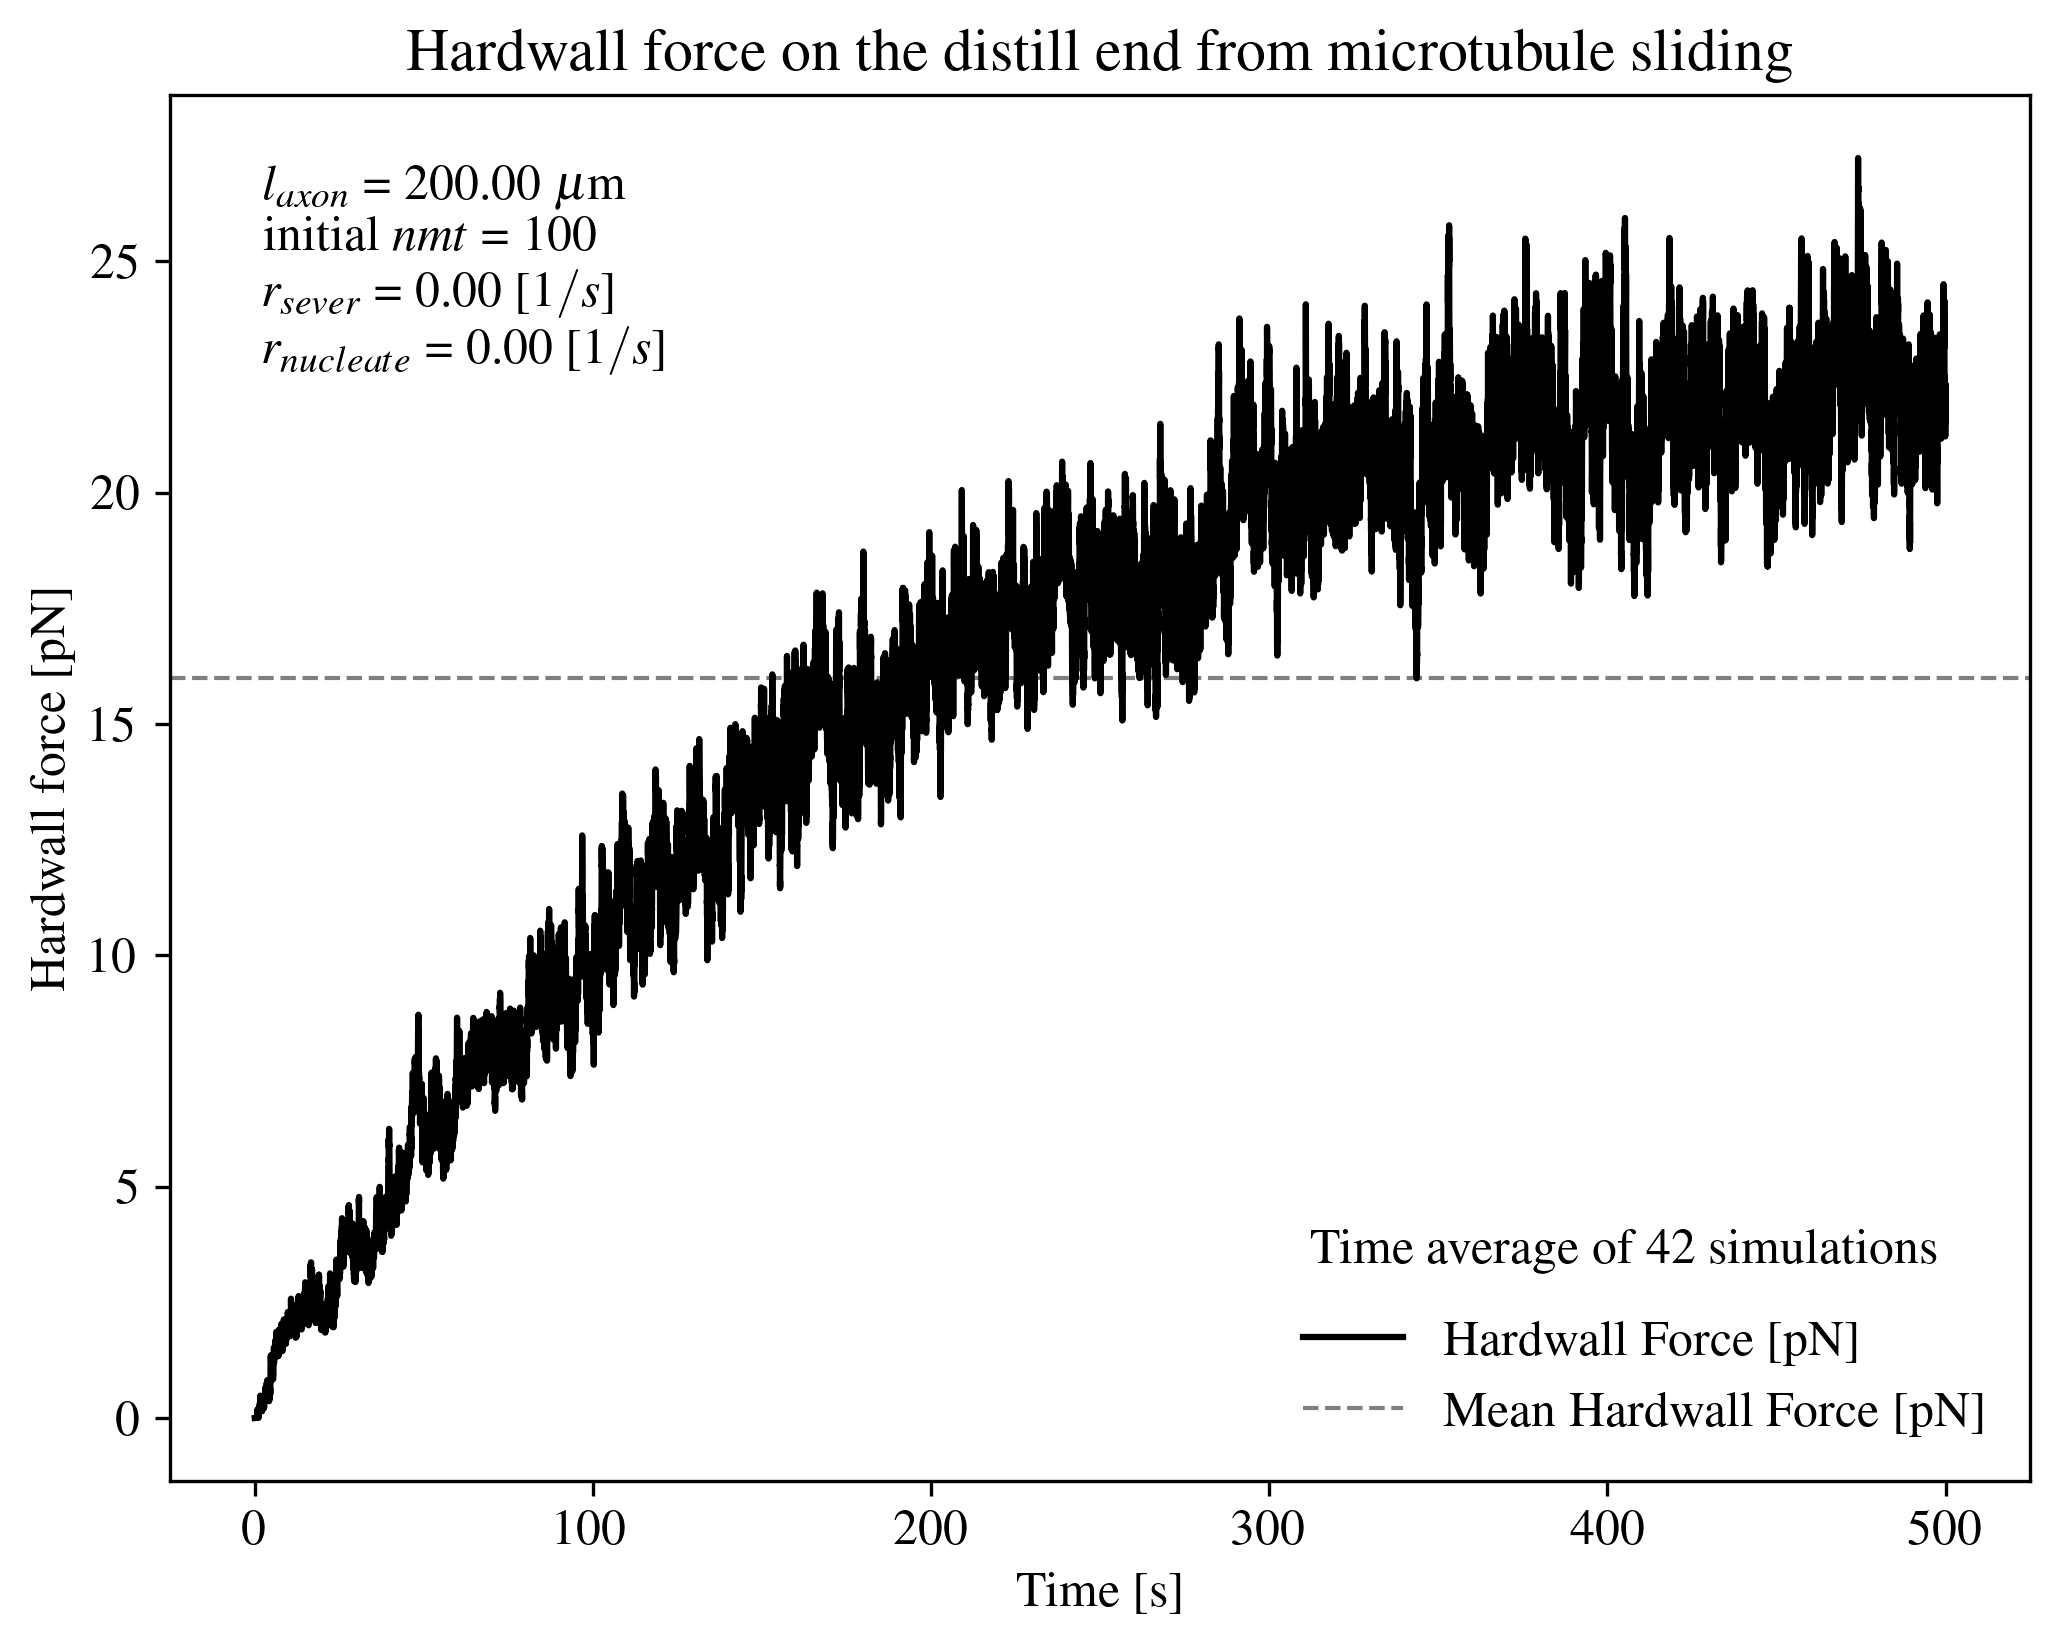
\includegraphics[width=0.4\textwidth]{figures/preliminary_force/hforce_hardwallruns3.png}
    \caption{By recording the force applied to MTs at the distill end of the axon, summing at each time step, and averaging over many simulations, the above is produced.}
    \label{fig:prelim}
\end{figure}

Shown in Figure \ref{fig:prelim} is the force exerted on the distill end of the MT through previously investigated polarity sorting mechanisms only. The axon length and number of MTs remained constant throughout time in all simulations. The forces recorded are significant to the growth cone. 

\begin{figure}
    \centering
    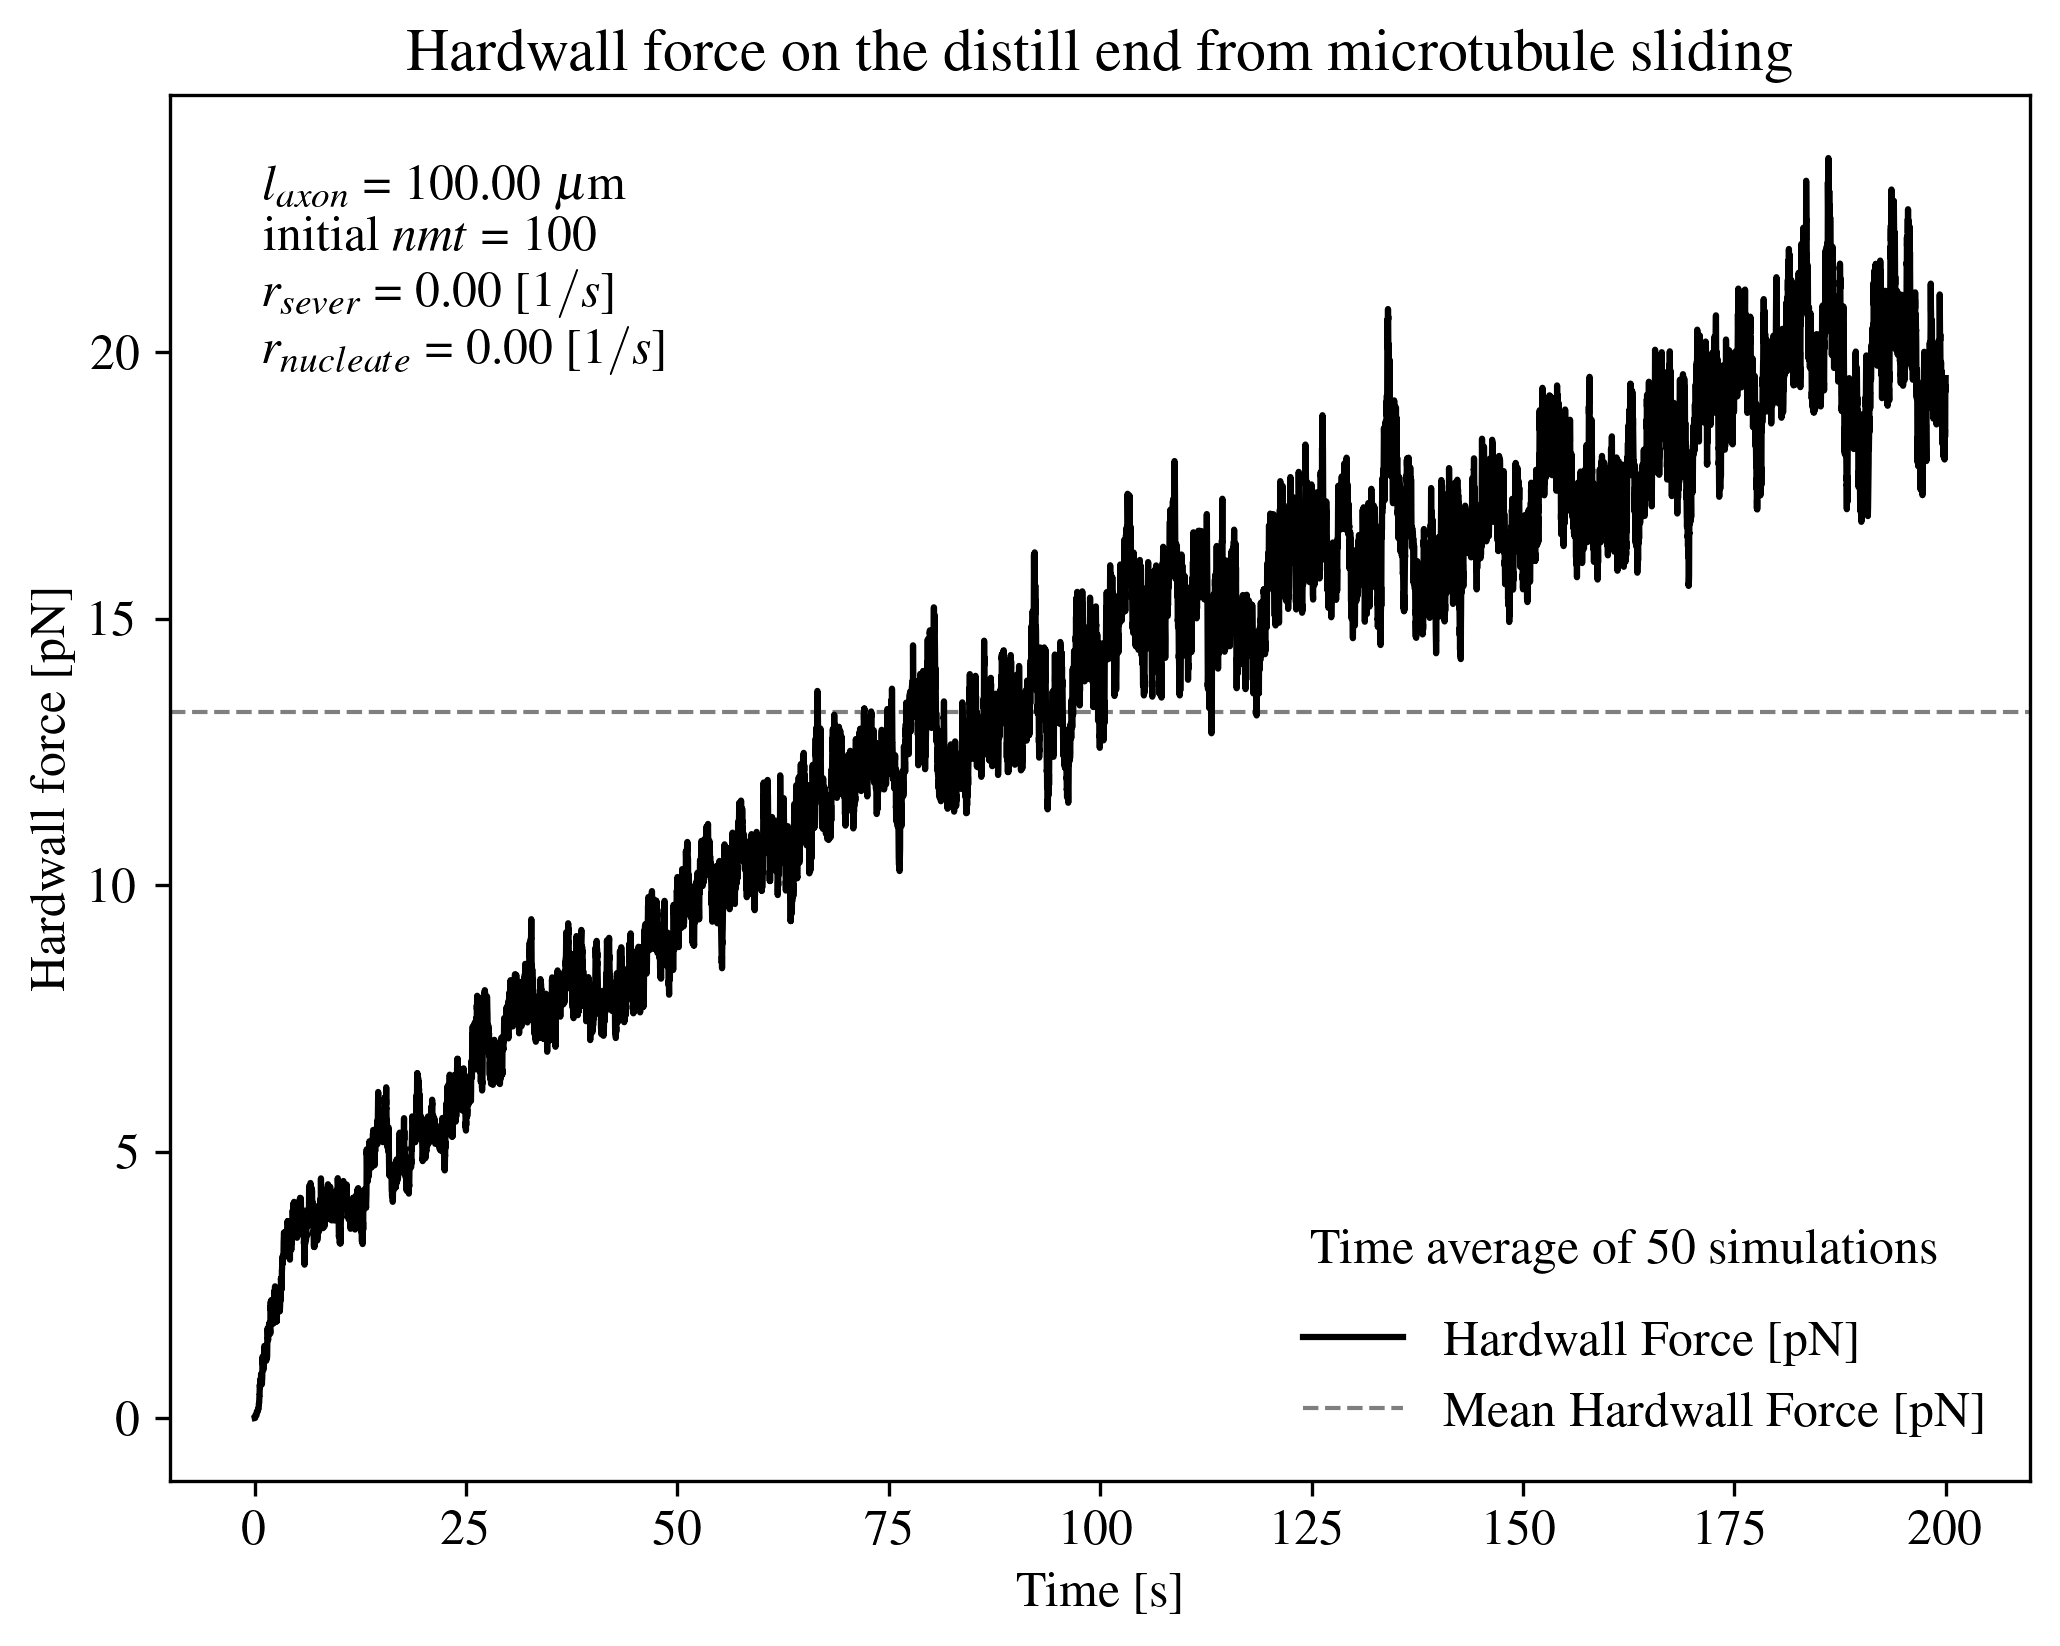
\includegraphics[width=0.4\textwidth]{figures/preliminary_force/hforce_hardwallrunsnonucsevlonger.png}
    \caption{The hardwall force on the distill end for a shorter axon.}
    \label{fig:long}
\end{figure}

Shown in Figure \ref{fig:long} is a similar force investigation but the length of the axon has been decreased. The forces at corresponding times to Figure \ref{fig:prelim} are higher implying the existence of a length dependence on ``sorting force''. A parameter sweep of length will need to be conducted to measure this length dependence. One possibility is that this length dependence means axons grow with microtubule force in the early stages of life and transition to a ``clutch'' mechanism, described in references, later on as they reach some critical length.

\infosection{Acknowledgements}
% people to include
\begin{itemize}
\item Members of CWU Biophysics Lab,
\item Dr. Peter Baas and Bridie Eckel of Drexel University,
\end{itemize}
Work for this project was supported by NSF Research at Undergraduate Institutions Award 1915477.

% bibliography here (IF I HAD ONE)
\infosection{Fake bibliography}
I referenced a lot of papers but couldn't figure out the Zotero \LaTeX\ integration.
\begin{itemize}
\item The 4-ish papers sent to me to read about axon growth dynamics
\item The several citations present on my WA-AAPT poster, also on the BPS poster
\item There are some more papers in my Zotero library that I may be pulling information from without realizing.
\end{itemize}
\end{document}
